\documentclass{article}

% if you need to pass options to natbib, use, e.g.:
% \PassOptionsToPackage{numbers, compress}{natbib}
% before loading nips_2016
%
% to avoid loading the natbib package, add option nonatbib:
% \usepackage[nonatbib]{nips_2016}

\usepackage[final]{nips_2016}

% to compile a camera-ready version, add the [final] option, e.g.:
% \usepackage[final]{nips_2016}

\usepackage[utf8]{inputenc} % allow utf-8 input
\usepackage[T1]{fontenc}    % use 8-bit T1 fonts
\usepackage{hyperref}       % hyperlinks
\usepackage{url}            % simple URL typesetting
\usepackage{booktabs}       % professional-quality tables
\usepackage{amsfonts}       % blackboard math symbols
\usepackage{nicefrac}       % compact symbols for 1/2, etc.
\usepackage{microtype}      % microtypography
\usepackage{graphicx}       % include graphics
\usepackage{subcaption}     % subfigures
\usepackage{algorithm}
\usepackage[noend]{algpseudocode}

\graphicspath{ {images/} }


\title{Deep reinforcement learning for Snake}

\author{
  Louis Martin \\
  \texttt{louis.martin@student.ecp.fr} \\
  \And
  Pierre Stock \\
  \texttt{pierre.stock@student.ecp.fr} \\
}

\begin{document}

\maketitle

\begin{abstract}
  Reinforcement Learning is a very active machine learning field inspired by behavioral psychology, consisting in giving rewards to agents interacting with environments to encourage them to take the right action in a given context.
  Applying Deep Learning techniques such as Convolutional Networks (CNNs) to Reinforcement Learning led to Deep Reinforcement Learning and some major recent successes such as beating world-class professional players to the game of Go \cite{silver2016go} or playing Atari 2600 games \cite{mnih2013playing}.
  We will focus on applying policy gradients networks, a conceptually simple framework that uses asynchronous gradient descent for optimization of deep neural network controller to play the game of Snake \cite{mnih2016asynchronous}.
\end{abstract}

%% Abstract (½ page):
%% What problem(s) is studied ?
%% Why is it relevant ?
%% What solution(s) is proposed ?
%% Which contributions (theory, numerics, etc) ?
\section{Introduction}
%% Introduction (~3 pages) :
%% Presentation of the problem(s).
%% Previous works (at least a few citations). If relevant, include things that you have seen during the MVA course (or possibly other courses).
%% Contributions. Why is the studied method different/better/worse/etc. than existing previous works.
One of the first successful end-to-end reinforcement reinforcement learning algorithm applied games was TD-Gammon \cite{tesauro1995temporal}.
The algorithm achieved Super-human performance more than 20 years ago.
Even neural networks were already used in reinforcement learning in \cite{lin1993reinforcement} in 1993.
However with the ever-improving computational capabilities and the recent revival of interest in convolutional networks since \cite{krizhevsky2012imagenet}, it has been possible to design new algorithms achieving remarkable results using only visual data.

  Working with high dimensional data such as raw images proves to be a very difficult problem that was usually handled by designing tailor-made low dimensional features that would represent the environment as accurately as possible.
 Deep learning allows to handle this problem thanks to its millions of parameters and translation invariant convolutions that can convert an image into more and more abstract features as you go deeper in the layers.
The algorithm can therefore be end-to-end with no need to handcraft problem-specific features.
 This led to the success of \cite{bellemare2012arcade} by DeepMind technologies, that played seven Atari 2600 games at human-level performance and even better.
They followed up 3 years later with \cite{mnih2015human} with a deep Q-network agent that was able to surpass humans at 49 different games using the exact same model for each, which showed its adaptability.

% TODO: Policy gradent > Q-learning, that's why we used it
They later on showed in \cite{mnih2016asynchronous} that using policy networks performed even better that deep Q-learning, and we will follow their path in this report.

Policy gradients can be used with other models such as Monte Carlo Tree Search (MCTS), which was brilliantly illustrated by AlphaGo which beat the world champion at the game of Go \cite{silver2016go}.

We are going to focus on learning the retro game called snake.
One great aspect of training reinforcement algorithms on games is that the environment can be completely simulated and its complexity controlled.
This can therefore be seen as a playground and preparation for more difficult "real world" tasks.
One of the challenges that we have to solve when playing games is the delay between actions and resulting rewards and the correlation between successive action.
Many ideas where used in order to mitigate this problem including experience replay \cite{lin1993reinforcement} or delayed mini batch training.

In our special case we are going to play snake using policy gradients with delayed mini batch training.



\section{Deep Reinforcement Learning}
%% Main body (~10 pages) :
%% Presentation of the method(s).
%% Theoretical guarantees.

\subsection{Notations and background}

Our agent is the snake from the well-known eponymous game. It interacts with the environment $\mathcal E$ to gets its current state $s_t$ which is a $N \times N$ grid. The initial state at the beginning of one game $s_0$ is the following: the snake has a length of 3 pixels and starts from the left-upper corner of the grid, its head being the rightmost part of its body and a fruit appears randomly in one pixel of the grid where the snake is not (see Fig \ref{snake_init}). Note that the fruit does not disappear until the snake has eaten it. The goal of the game is to eat as many fruits as possible in one game.

\begin{figure}[!htpb]
\centering
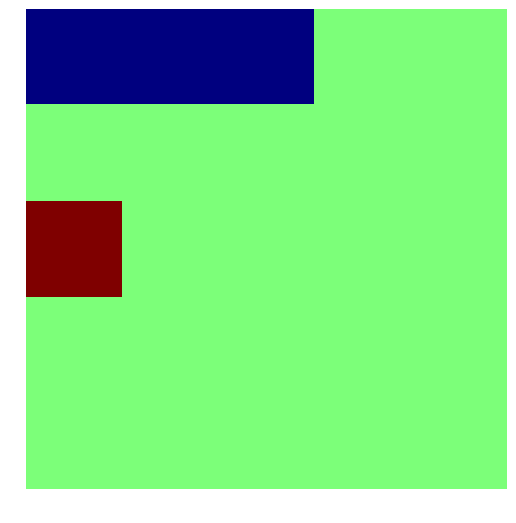
\includegraphics[width=.4\linewidth]{snake_initial_state.png}
\caption{Initial state of the game for $N = 5$}
\label{snake_init}
\end{figure}

At each time $t$, the agent selects an action $a_t$ from the set of actions is $\mathcal A =$ \{up, down, left, right\}. Each action $a_t$ modifies the state of the game and triggers a reward $r_t$ according to the following rules:

\begin{itemize}
\item The snake will eat itself after $a_t$. Game over, get the associated reward $r_{{eat}}$.
\item The snake will hit a wall after $a_t$. Game over, get the associated reward $r_{{hit}}$.
\item The snake will eat a fruit after $a_t$. Move according to $a_t$, get the associated reward $r_{{fruit}}$, grow snake by 1 pixel at the bottom (the opposite of the head), generate one fruit in a random location of the grid where the snake body is not.
\item Otherwise. Move according to $a_t$, get the associated reward $r_{{nothing}}$.
\end{itemize}

For the sake of clarity, we will first use the set of rewards

\begin{center}
\{{eat}: $-10$, {hit}: $-10$, {fruit}: $+10$, {nothing}: $-1$\}
\end{center}

that we will carefully tune later. Thus, we strongly encourage fruit eating, strongly discourage wall hitting and self-eating and slightly discourage doing nothing to avoid undesirable behaviors such as infinite looping.

We make the standard assumption that the rewards are discounted by a factor $\gamma \in [0, 1[$ and define the expected return at time $t$ in a game of length $T$ as

\[R_t = \sum_{t' = t}^T \gamma^{t' - t} r_{t'}\]

Using this notion, we can express the goal of the game more formally: the goal of the agent is to \textit{maximize the expected return} from each state $s_t$ by computing the optimal policy $\pi^{\star}$.

The policy, that we denote $\pi$,
maps each state of the game $s_t$ to a distribution over the action state $\mathcal A$. This means that $\pi_t \in [0, 1]^{|A|} = [0, 1]^4$ where $\pi_{t,i}$ denotes the probability of taking action $\mathcal A_i$ given the state $s_t$.

\subsection{Policy Networks}

This algorithm is based on the algorithm described in \cite{mnih2016asynchronous}.

Our agent will be implemented by a policy network that will take the state of the game $s_t$ as input and output 4 probabilities corresponding to the policy $\pi_t$. For the network to be able to detect motion (and where the head of the snake is), we actually feed it with the last two frames $(s_{t-1}, s_t)$, where $s_{-1}$ is the grid filed with zeros.

We first experimented a fully connected network with 1 hidden layer of size $n_h$, taking as input $2 * N^2$ pixels and outputting $4$ values, stacked with a softmax layer to output probabilities. The structure of this network is illustrated in Fig \ref{network}. In this example, the network will output very low probabilities for going up (eating itself) or going down (hitting the wall), and will be more likely to go to the left than to the right due to the presence of the fruit on the right side, and because going to the left will definitely lead to game over.

\begin{figure}[!htpb]
\centering
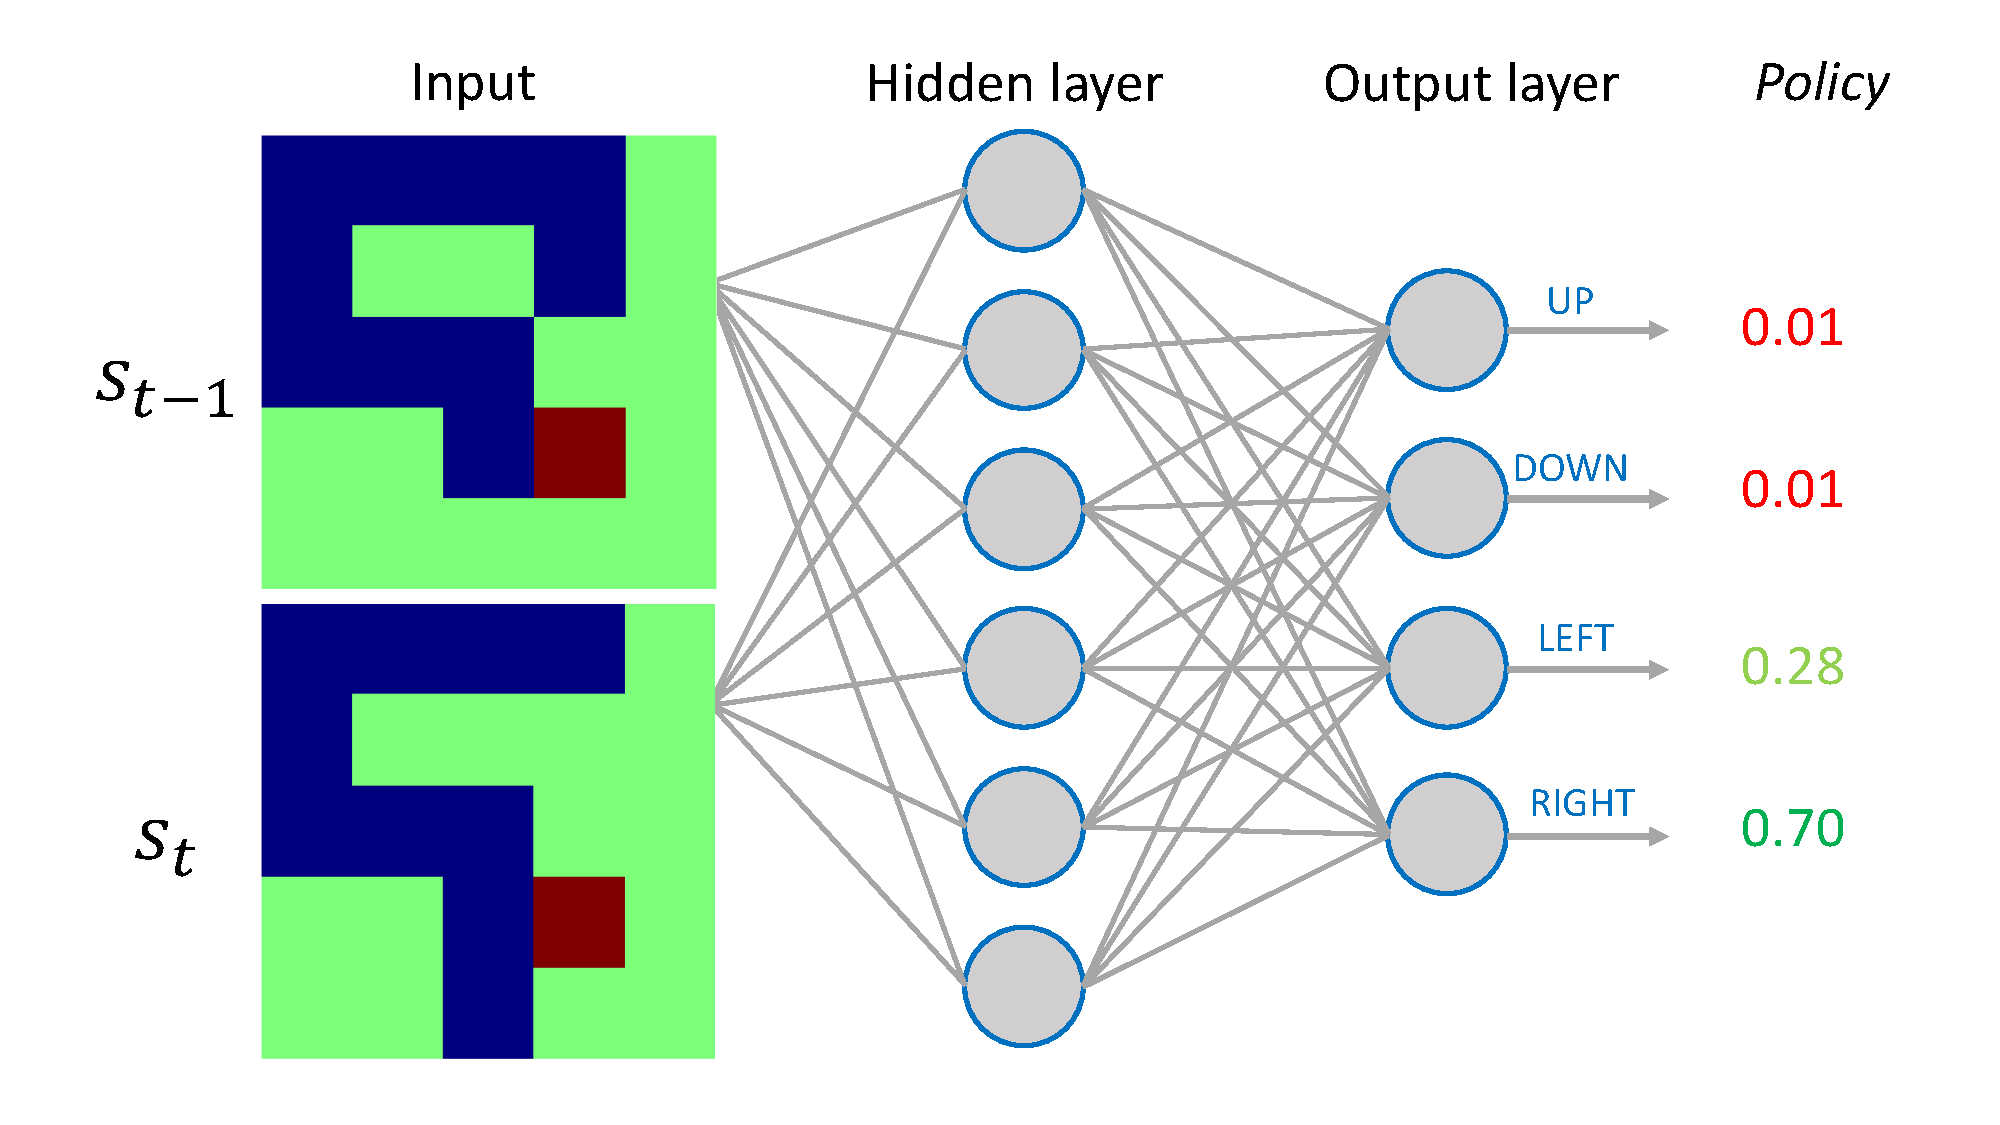
\includegraphics[width=\linewidth]{layer.pdf}
\caption{Initial state of the game}
\label{network}
\end{figure}

The training goes as follows. After initializing the network, we play a first game by successively feeding the tuple of the last two states $(s_{t-1}, s_t)$ to the policy network (forward pass), sampling action $a_t$ from the output probabilities and updating the new state of the game $s_{t + 1}$ until the game is over.

We repeat this procedure for a batch of $n_b$ games while storing the output probabilities and the sampled actions. Then, we want to update the parameters of the network by backpropagation so that our network actually learns to play better for the next batch.

To do that, we have to define a loss function assessing whereas a particular action $a_t$ in a particular game  of the batch was rather \textit{good} or \textit{bad}. Let us note $x_{i, t} = (s_{i, t - 1}, s_{i, t})$ where $s_{i,t}$ is the state of the $i^{th}$ game of the batch at time $t$, $y_{i, t}$ the action that was sampled from the policy network after the forward pass of $x_{i, t}$ and $R_{i, t}$ the expected return at time $t$ of the action $y_{i, t}$, that is,

\[R_{t, i} = \sum_{t' = t}^{T_i} \gamma^{t' - t} r_{t'}\]

where $T_i$ is the length of the $i^{th}$ game. Then, the loss function for that particular batch $k$ writes

\[\ell_k = - \sum_{i = 1}^{n_b} \sum_{t = 1}^{T_i} R_{i, t} \log p(y_{i, t} | x_{i, t})\]

where $p(y_i | x_i)$ is the probability of action $y_i$ given by the network when it sees input $x_i$. Note that the loss function \textit{varies} from batch to another to adapt to the games that were played.

The number $R_{t, i}$ is usually referred to as the \textit{advantage} of the game $i$ at time $t$. Note that $R_{t, i}$ depends on the discount factor $\gamma$. Low values of $\gamma$ will lead to \textit{short-sighted} policies whereas high values of lambda will lead to \textit{long-sighted} policies.

Note that the reason we don't backpropagate right after the forward pass of an action is that we're not sure yet if this action will be \textit{good} or \textit{bad}, thus we wait until the end of the game to decide that (see definition of the expected return).

Note also that we normalized the expected rewards $R_{i, t}$ for each batch, which has two major advantages:
\begin{itemize}
\item It helps diminish the variance of the gradient when backpropagating and thus ensures a more stable learning process
\item It tells the network that roughly half of the games of the batch were rather \textit{bad}, whereas the other half games were rather \textit{good}. This is of course not the case in practice but this has significantly improved our experimental results.
\end{itemize}

The pseudocode for this algorithm is detailed below.

\begin{algorithm}
\caption{Learning algorithm}\label{algo}
\begin{algorithmic}[1]
\Statex Randomly initialize network weights $\theta^0$
\Statex Initialize network gradients $d\theta = 0$
\Statex \textbf{for} $j = 1$ .. \#iterations \textbf{do}
\Statex ~~~~ \textbf{for} $i = 1$ .. $n_b$ \textbf{do}
\Statex ~~~~ ~~~~ play game $i$
\Statex ~~~~ ~~~~ store corresponding expected returns $(R_{i, 1}, \dots R_{i, T_i})$
\Statex ~~~~ ~~~~ store corresponding probabilities $\log p(y_{i, t} | x_{i, t})$
\Statex ~~~~ \textbf{end}
\Statex ~~~~ compute loss $\ell_j$
\Statex ~~~~ update network parameters $\theta^{j+1} = \theta^j -  \eta \frac{\partial \ell}{\partial \theta}$
\Statex \textbf{end}
\Statex\textbf{return} network parameters $\theta$
\end{algorithmic}
\end{algorithm}

\section{Results}
\subsection{Fully connected neural network}
Our implementation in Python of a snake environment and of the algorithm detailed above is available online\footnote{GitHub repo: \url{http://github.com/RLSnake/Snake}}{}.

We implemented a fully connected neural network to begin with and after some tinkering, it led to a model that fully learned how to play the snake.

We ran a set of experiments on the network structure defined above while studying the impact of the main parameters\footnote{Illustrated notebook: \url{http://github.com/RLSnake/Snake/blob/master/snake/parameter_exploration.ipynb}}{}.
Each set of parameters was run for 10.000 games (20.000 for the batch size).
We experimentally observed that the inter-training variability was small so we ran each set of parameter only once to get good qualitative results.

Our performance measure for the snake is the number of time it played without loosing called \textbf{lifetime}, along with the number of fruits eaten.
In order to prevent the lifetime measure to be impacted by a algorithm that would loop over to avoid the walls without actually trying to eat the fruit, we set a constraint on the time spent without eating fruits.
If the Snake did not eat any fruit for $3 \times grid\_size$ actions, it lost the game. This ensures that the snake has to eat fruits in order to keep playing a get a higher reward.

Parameters: learning rate, set of rewards, $n_h$, $n_b$, $N$, $\gamma$. Trained for $x$ iterations = x games.

\subsubsection*{Batch size}

\begin{figure}[!htpb]
\centering
  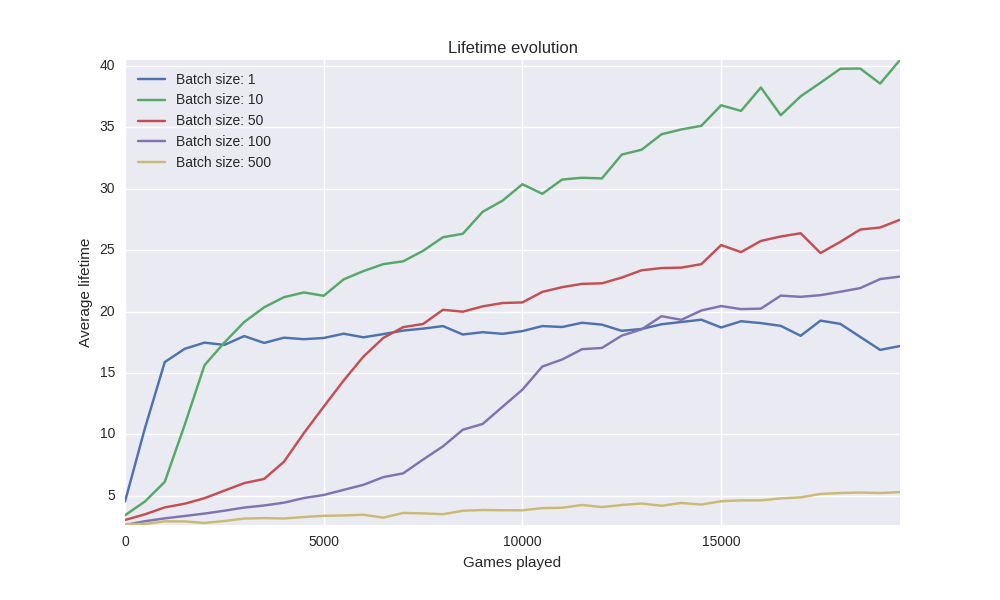
\includegraphics[width=.8\linewidth]{batch_size_dependence.png}
  \caption{Influence of the batch size}
  \label{batch_size}
\end{figure}

The batch size $n_b$ is a critical parameter because it determines how often we update the network.
It is directly linked with the exploitation-exploration trade off.
Figure \ref{batch_size} gives us interesting insights on the influence of the batch size.
The smaller the batch size, the faster the algorithm learns to play. However it seems that higher batch sizes are slower to get running but then have higher and steady performance increase.
It can be explained by the fact that small batch size pushes the algorithm to exploit the first solution it found to have a high reward and therefore being stuck. Higher batch size allow the network to see more use cases and then to derive the best action.

It is here interesting to note that $n_b = 10$ gives the best compromise: it learns fast and then steadily increases its performance with a good slope.

\subsubsection*{Hidden units}

\begin{figure}[!htbp]
\centering
  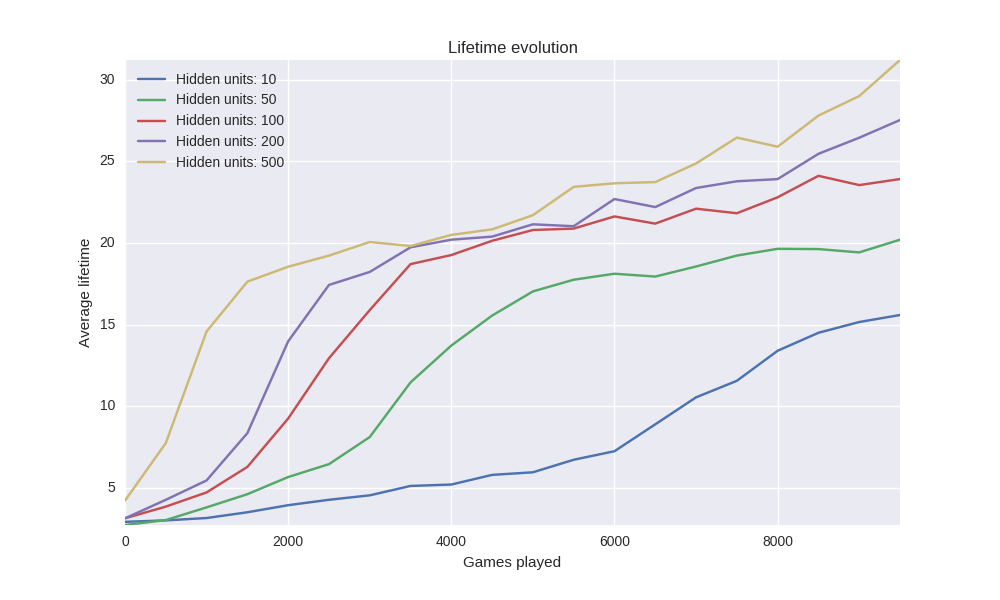
\includegraphics[width=.8\linewidth]{hidden_units_dependence.png}
  \caption{Influence of the number of hidden units}
  \label{hidden_units}
\end{figure}

Our fully connected is only one layer deep so we can tune just one parameter for simplicity.
Figure \ref{hidden_units} confirms our intuitive guess that larger number of hidden units leads to better performance thanks to more parameters and thus more representational power.
However the increase in performance does not linear in number of hidden units, and we don't want to much units to prevent over-fitting.
Another interesting findings is that the computational time does not increase linearly with the number of hidden units which is somewhat counter intuitive. Maybe the tensorflow implementation is more efficient for a higher number of hidden units.

\subsubsection*{Number of frames fed to the network}

\begin{figure}[b]
\centering
  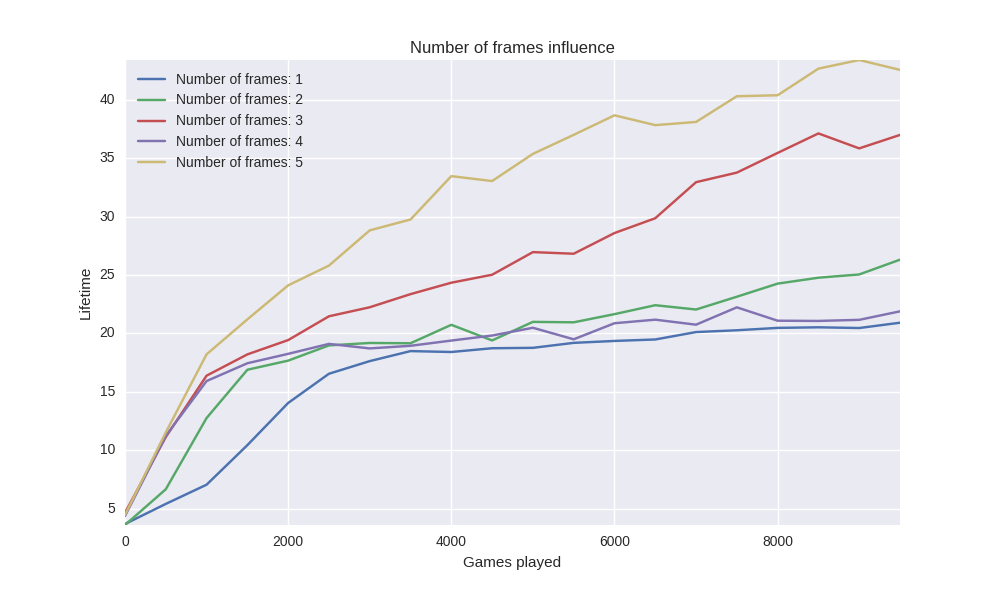
\includegraphics[width=.8\linewidth]{number_of_frames_dependence.png}
  \caption{Influence of the number of frames fed to the network}
  \label{number_of_frames}
\end{figure}

We are now studying the time dimension for the training that is represented by the number of consecutive frame that we feed through the network.
It is a bit less clear if the number of frames has a strong influence on the performance on figure \ref{number_of_frames}.
It nevertheless seems to increase with the number of frame which is what we could have guessed. More frames means more information but also more parameters to model the problem.
% TODO: link to notebook

\subsubsection*{Analysing the model behaviour}

\begin{figure}[!htpb]
\centering
  \begin{subfigure}[b]{.19\linewidth}
    
\includegraphics[width=\linewidth]{snake_61.png}
  \end{subfigure}
  \begin{subfigure}[b]{.19\linewidth}
    
\includegraphics[width=\linewidth]{snake_62.png}
  \end{subfigure}
  \begin{subfigure}[b]{.19\linewidth}
    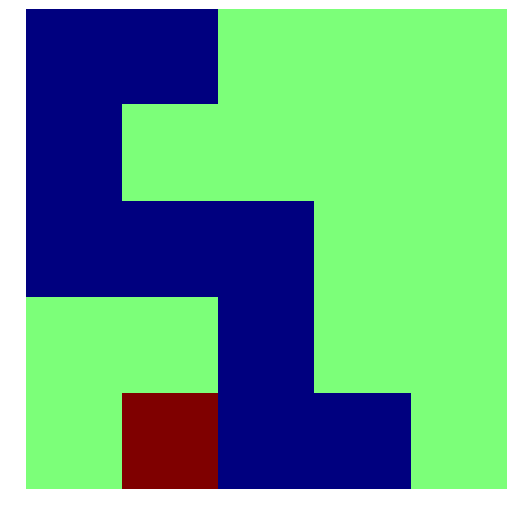
\includegraphics[width=\linewidth]{snake_63.png}
  \end{subfigure}
  \begin{subfigure}[b]{.19\linewidth}
    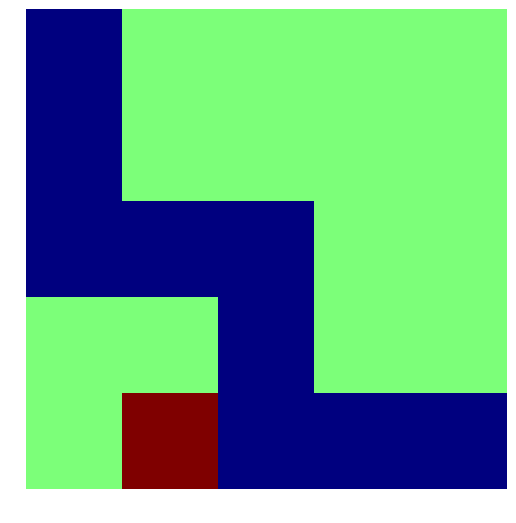
\includegraphics[width=\linewidth]{snake_64.png}
  \end{subfigure}
  \begin{subfigure}[b]{.19\linewidth}
    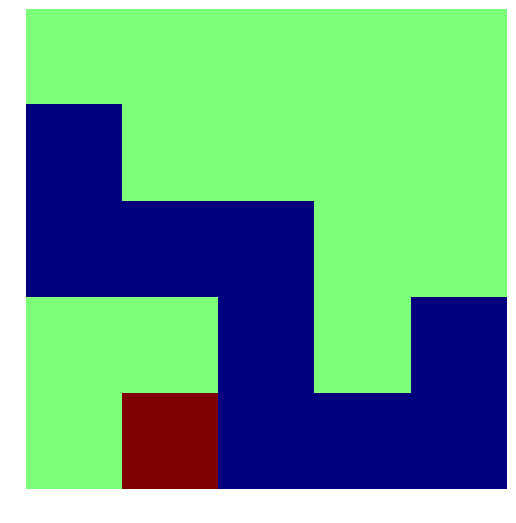
\includegraphics[width=\linewidth]{snake_65.png}
  \end{subfigure}
   \begin{subfigure}[b]{.19\linewidth}
    
\includegraphics[width=\linewidth]{snake_66.png}
  \end{subfigure}
  \begin{subfigure}[b]{.19\linewidth}
    
\includegraphics[width=\linewidth]{snake_67.png}
  \end{subfigure}
  \begin{subfigure}[b]{.19\linewidth}
    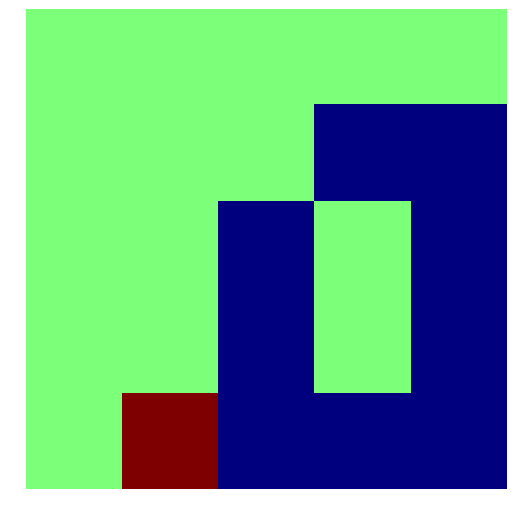
\includegraphics[width=\linewidth]{snake_68.png}
  \end{subfigure}
  \begin{subfigure}[b]{.19\linewidth}
    
\includegraphics[width=\linewidth]{snake_69.png}
  \end{subfigure}
  \begin{subfigure}[b]{.19\linewidth}
    
\includegraphics[width=\linewidth]{snake_70.png}
  \end{subfigure}
  \begin{subfigure}[b]{.19\linewidth}
    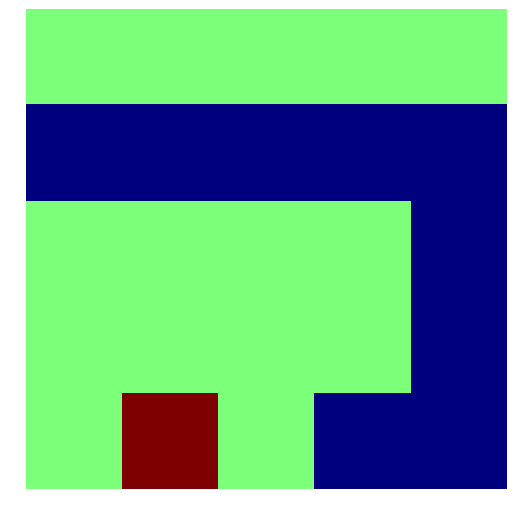
\includegraphics[width=\linewidth]{snake_71.png}
  \end{subfigure}
  \begin{subfigure}[b]{.19\linewidth}
    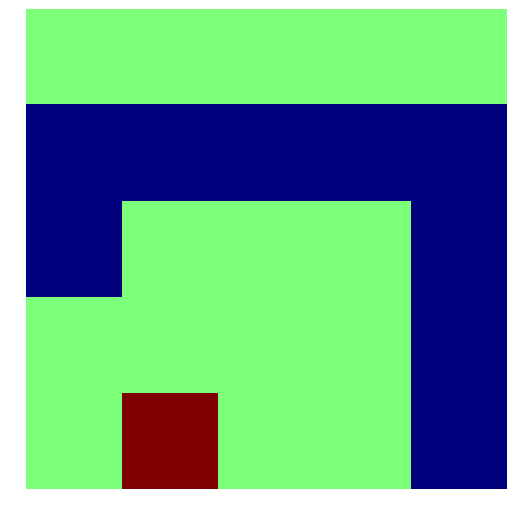
\includegraphics[width=\linewidth]{snake_72.png}
  \end{subfigure}
  \begin{subfigure}[b]{.19\linewidth}
    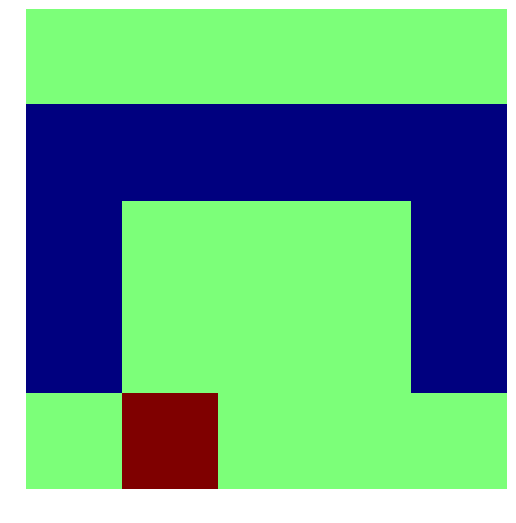
\includegraphics[width=\linewidth]{snake_73.png}
  \end{subfigure}
  \begin{subfigure}[b]{.19\linewidth}
    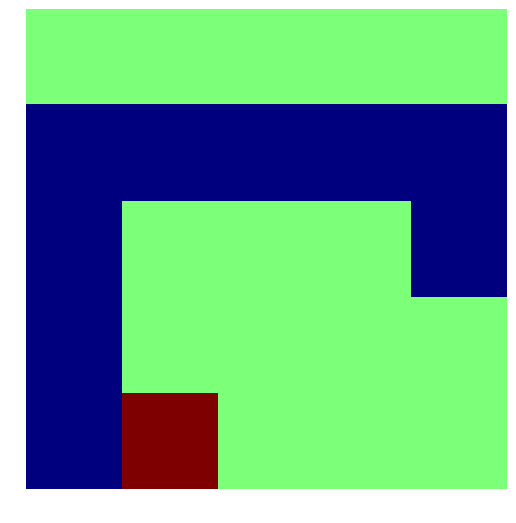
\includegraphics[width=\linewidth]{snake_74.png}
  \end{subfigure}
  \begin{subfigure}[b]{.19\linewidth}
    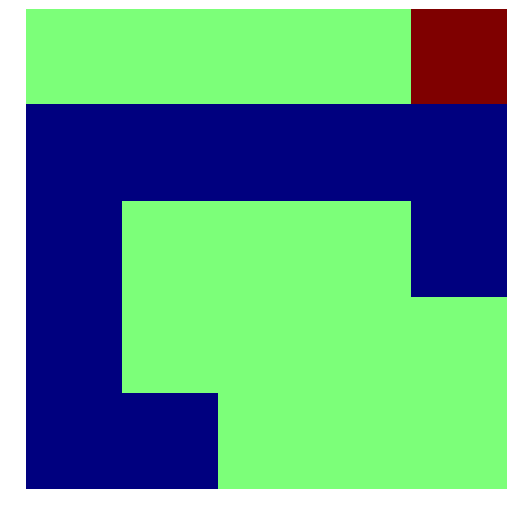
\includegraphics[width=\linewidth]{snake_75.png}
  \end{subfigure}
  \caption{The snake learns to take as much space as possible in order to avoid being stuck}
  \label{snake_behaviour}
\end{figure}

While we tried to improve the training and our model, we watched the algorithm interact with the environment.
We witnessed some interesting behaviors.
The algorithm often proceeds in two intuitive steps, first it tries to avoid the walls and only after it tries to eat fruit.
This is why our experiment may be questioned. The number of games played might be too small to clearly reflect the two steps. The experiments probably happen mainly during the "Avoiding the wall" part in which smaller models can succeed easily for example.

We also noticed that the algorithm learnt to occupy as much space as possible to avoid being stuck. We observed in figure \ref{snake_behaviour} that the snake did not rush to get the fruit but rather went the other way not to get stuck.

\subsection{Convolutional neural network}

Fully connected neural networks are not the optimal bet because they are in a way over-fitting the environment and learning lots of states.
Their big problem is that each parameter is assigned to one pixel.
As a consequence their number of parameter does not scale at all to larger images and most importantly they cannot reuse something that they learnt in a part of the image to another part of the image.
In other words, they are not translation invariant.
That is why convolutional neural network are way more adapted to this kind of data.
Our implementation allowing to easily change the network structure, we tried CNN models on this problem.
At the time being, we didn't have a sufficient computational time to run all the experiment to wanted.

The convolutional network passed the "Avoiding the wall" test but did not understand that it had to eat fruit.
It remains an open issue that requires further investigation.

\section{Conclusion}
%% Conclusion and perspective (~1 page)
%% Summary of the result obtained: pros and cons (limitation, problems, error in the articles, etc)
%% Possible improvement/extension

Applying deep policy networks to the game of Snake, we have shown that Deep Reinforcement techniques yield promising results to play games which require good reflexes and a bit of a long-time strategy (eating fruits, not being cornered and stuck while the snake keeps growing).

After training over thousands of games, our snake begins to eat fruits consistently until it grown too much and is eventually stuck by its own body.

These techniques pave the way to real-world applications involving robots opening doors or walking for example.

% bibliography
\newpage

\bibliographystyle{unsrt}
\bibliography{bibliography}

\end{document}
